\section{Corridas}

La cámara que tomo como referencia es la número 0, la cámara que va adelante
es la cámara 4 y la que va atrás es la cámara 1. Esto lo veo siguiendo el orden
de los picos de presión.

\subsection{Iteración 1}
La geometría a evaluar es:

\begin{tabular} { | c c c c c c c c c| }
    \hline
    caso    & dta   & dte    & length intake tube & length exhaust tube & iia   & ifa    & eia    & efa    \\
    $run_4$ & 97.24 & 81.154 & 519.305            & 876.66              & 1.118 & 70.153 & 85.144 & 11.129 \\
    \hline
\end{tabular}

El ángulo que se ve en los diagramas de alzada sigue el centro del aspa
entonces para $584-600 = -16^{\circ}$, comienza a abrir el puerto.

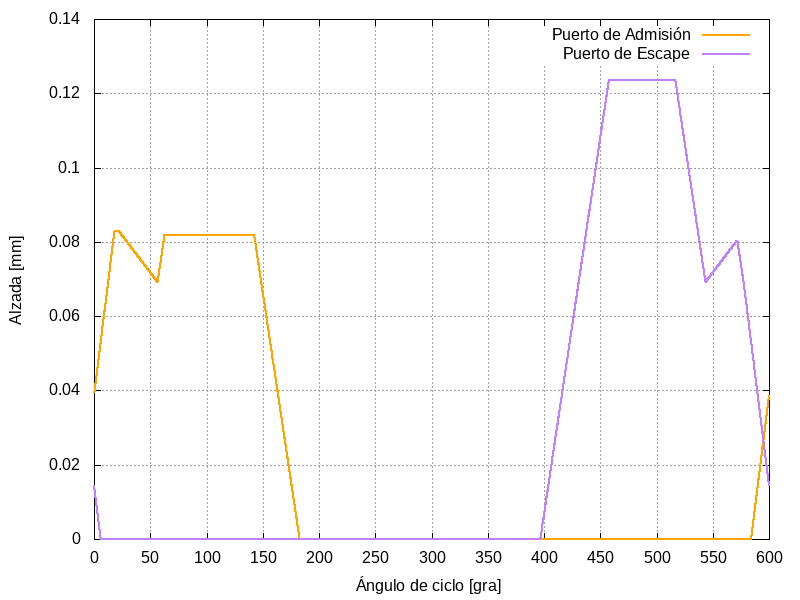
\includegraphics{alzadas_corrida_1.png}

\subsubsection{Admisión}

Datos para generar geometría y calcular condiciones de borde para el puerto de admisión.

\begin{tabular}{ | c c c c c c c c c c c c c c c c c c | }
    \hline

    RPM  & $\theta$ & $L_v$  & $\rho_4$     & $\rho_0$     & $\rho_1$     & $\rho_I$     & $\rho_E$     & $P_4$       & $P_0$       & $P_1$       & $P_I$       & $P_E$       & $T_4$       & $T_0$       & $T_1$       & $v_I$       & $v_E$ \\
    7000 & 586.02   & 4.776  & 0.6821053701 & 0.3624584994 & 0.2599165095 & 0.9996209217 & 0.2657775677 & 81176.70548 & 63045.63922 & 63912.41539 & 86544.50137 & 62104.69409 & 414.6656457 & 606.058948  & 856.7802916 & 124.2366931 & 75.38037424
    7000 & 10.084   & 63.154 & 0.9043294104 & 0.8346255683 & 0.4937075062 & 1.299845405  & 0.5110165623 & 112734.4691 & 125520.0146 & 155196.8985 & 117962.4246 & 164535.9801 & 434.3583473 & 524.009788  & 1095.295772 & 106.1404863 & 0
    7000 & 80.00    & 81.937 & 1.66296226   & 0.560047667  & 0.499083616  & 0.651666142  & 0.208396404  & 245212.343  & 62998.4550  & 117080.480  & 63317.6542  & 53859.2916  & 513.78099   & 391.943087  & 817.389934  & 28.4532634  & 0 \\
    7000 & 95.073   & 81.937 & 2.159126886  & 0.5648368521 & 0.3970975168 & 0.7808796925 & 0.2198742509 & 350898.8852 & 64557.6244  & 75394.08427 & 69659.85383 & 52511.57087 & 566.2678777 & 398.2379284 & 661.5431893 & 114.8868588 & 0
    7000 & 115.09   & 81.937 & 3.441492961  & 0.7642406441 & 0.5949980691 & 1.079478992  & 0.3852977456 & 662137.2556 & 92694.90095 & 93569.64723 & 93129.45462 & 108700.5503 & 670.3772106 & 422.613939  & 547.9457201 & 137.6560695 & 0 \\

\end{tabular}

\begin{description}
    \item [$\theta$] Es el ángulo del ciclo
    \item [Lv] Es una alzada ficticia para calcular un área de cortina equivalente al área descubierta del puerto
    \item [4] Representa una cámara anterior a la que se está evaluando
    \item [0] Representa la cámara que se está evaluando
    \item [1] Representa una cámara posterior a la cámara que se está evaluando.

\end{description}

\subsubsection{Escape}

Datos para generar geometría y calcular condiciones de borde para el puerto de escape.


\begin{tabular}{ | c c c c c c c c c c c c c c c c c c | }
    \hline

    RPM  & $\theta$ & $L_v$   & $\rho_4$     & $\rho_0$     & $\rho_1$     & $\rho_I$     & $\rho_E$     & $P_4$       & $P_0$       & $P_1$       & $P_I$       & $P_E$       & $T_4$       & $T_0$       & $T_1$       & $v_I$       & $v_E$ \\
    7000 & 400.09   & 6.786   & 0.4397398556 & 1.653849648  & 9.634195732  & 1.712592508  & 0.2055229342 & 117402.434  & 927559.9819 & 3057396.949 & 168606.6737 & 114909.6386 & 930.2493486 & 1954.177828 & 1105.74368  & 0           & 140.1007097 \\
    7000 & 450.22   & 108.568 & 0.4257464033 & 0.3234929103 & 9.005108648  & 0.839020506  & 0.306306707  & 85779.62163 & 92040.47343 & 9163815.16  & 81067.63487 & 81910.96057 & 702.0228398 & 991.3617996 & 3545.728408 & 0           & 154.1017728 \\
    7000 & 490.01   & 123.601 & 0.8190572911 & 0.4940292948 & 3.039180562  & 1.679099565  & 0.4879958105 & 125209.7752 & 155412.4827 & 2133465.669 & 164536.5654 & 155285.7811 & 532.6501559 & 1096.10283  & 2445.948222 & 0           & -34.88813497 \\
    7000 & 550.01   & 71.872  & 0.6675997251 & 0.5855578823 & 0.61381122   & 0.7698783943 & 0.3894625003 & 79096.47107 & 159212.2521 & 235625.7297 & 83569.25204 & 135647.7192 & 412.8184147 & 947.3811895 & 1337.53758  & 0           & 312.420183 \\
    7000 & 599.93   & 15.227  & 0.8011871998 & 0.727449752  & 0.3712945437 & 1.14215585   & 0.374638127  & 97263.40568 & 107780.8682 & 104919.9599 & 99882.71658 & 105657.2501 & 422.9933828 & 516.2460966 & 984.5950585 & 129.2617544 & -57.28305258 \\

\end{tabular}
